\documentclass[a4paper, 11pt]{article}
\pdfoutput=1
\usepackage{jcappub}
% KP comment out the line below to get the table of contents back
\notoc{}

% KP test
\usepackage{feynmp-auto}
% before setting default graphics include widths, save the default to properly scale feynman diagrams with their labels
\makeatletter
\let\ginnatwidth\Gin@nat@width
\let\ginnatheight\Gin@nat@height
\makeatother
\setkeys{Gin}{width=\linewidth,totalheight=\textheight,keepaspectratio}
%if you don't use the feynmandiagram environment for feynmf/mp figures, and you've changed the Gin keys above, then you need to manually adjust the unit length for feynman diagrams to get ratio of tex labels to graphics right. \unitlength = 1.21mm for tufte \linewidth and \textheight
\DeclareGraphicsRule{*}{mps}{*}{}
\newenvironment{feynmandiagram}[1][]{\setkeys{Gin}{width=\ginnatwidth,totalheight=\ginnatheight}\begin{fmffile}{#1}
\begin{fmfgraph*}(100,70)\fmfpen{thick}}{\end{fmfgraph*}\end{fmffile}\setkeys{Gin}{width=\linewidth,totalheight=\textheight,keepaspectratio}}
% end feynman diagram setup

\usepackage{graphicx}
\usepackage{booktabs}
\usepackage{verbatim}
%\usepackage{caption} 
\usepackage{xspace}
\usepackage{hyperref}
\usepackage{multirow}
\usepackage{placeins}
\usepackage{array}
\usepackage{subcaption}

% KP test
\DeclareGraphicsRule{*}{mps}{*}{}
\setkeys{Gin}{width=\linewidth,totalheight=\textheight,keepaspectratio}

% Variables
\newcommand{\sigv}{\ensuremath{\langle \sigma v_{\rm{rel}} \rangle}\xspace}
\newcommand{\MET}{\ensuremath{E_T^\mathrm{miss}}\xspace}
\newcommand{\met}{\MET}
\newcommand{\MT}{\ensuremath{M_{T}}\xspace}
\newcommand{\pt}{\ensuremath{p_{T}}\xspace}

% Units
\newcommand{\GeV}{\textrm{GeV}\xspace}
\newcommand{\gev}{\GeV\xspace}
\newcommand{\TeV}{\textrm{TeV}\xspace}
\newcommand{\tev}{\TeV\xspace}

% Particle names
\newcommand{\lp}{\ensuremath{l^{+}}\xspace}
\newcommand{\lm}{\ensuremath{l^{-}}\xspace}
\newcommand{\ttbar}{\ensuremath{\bar{t}t}}
\newcommand{\bbbar}{\ensuremath{\bar{b}b}}
\newcommand{\A}{A}
\newcommand{\pa}{a}
\newcommand{\pH}{H}
\newcommand{\pZ}{Z}
\newcommand{\Hc}{\ensuremath{H^{\pm}}\xspace}

% Particle masses
\newcommand{\mDM}{\ensuremath{M_{\chi}}\xspace}
\newcommand{\mdm}{\ensuremath{M_{\chi}}\xspace}
\newcommand{\mmed}{\ensuremath{M_{\rm{med}}}\xspace}
\newcommand{\mMed}{\ensuremath{M_{\rm{med}}}\xspace}
\newcommand{\mZ}{\ensuremath{M_{\rm{Z}}}\xspace}
\newcommand{\mA}{\ensuremath{M_{A}}\xspace}
\newcommand{\ma}{\ensuremath{M_{a}}\xspace}
\newcommand{\mH}{\ensuremath{M_{H}}\xspace}
\newcommand{\mHc}{\ensuremath{M_{H^{\pm}}}\xspace}
\newcommand{\mh}{\ensuremath{M_{h}}\xspace}
\newcommand{\mt}{\ensuremath{M_{t}}\xspace}

% Couplings
\newcommand{\gDM}{\ensuremath{g_{\chi}}\xspace}
\newcommand{\gq}{\ensuremath{g_q}\xspace}
\newcommand{\gl}{\ensuremath{g_l}\xspace}
\newcommand{\gdm}{\gDM}
\newcommand{\ifb}{\ensuremath{\rm{fb}^{-1}}\xspace}

% Other parameters
\newcommand{\sinp}{\ensuremath{\sin\theta}\xspace}
\newcommand{\cosp}{\ensuremath{\cos\theta}\xspace}
\newcommand{\sinbma}{\ensuremath{\sin(\beta - \alpha)}\xspace}
\newcommand{\cosbma}{\ensuremath{\cos(\beta - \alpha)}\xspace}
\newcommand{\tanb}{\ensuremath{\tan\beta}\xspace}
\newcommand{\lap}[1]{\lambda_{P#1}} % can use like \lap1 , \lap2
\newcommand{\lam}[1]{\lambda_{#1}} % can use like \lam3

% Search channels
\newcommand{\metplusx}{\ensuremath{\MET+X}\xspace}
\newcommand{\hdm}{\ensuremath{h+\textrm{DM}}\xspace}
\newcommand{\monoh}{\ensuremath{h+\MET}\xspace}
\newcommand{\monohbb}{\ensuremath{h(bb)+\MET}\xspace}
\newcommand{\monoz}{\ensuremath{Z+\MET}\xspace}
\newcommand{\monozll}{\ensuremath{Z(\ell\ell)+\MET}\xspace}
\newcommand{\monozhad}{\ensuremath{Z(\textrm{had})+\MET}\xspace}

% Software/Program/Model names
\newcommand{\mg}{\textsc{MadGraph~5}\xspace}
\newcommand{\mgamcnlo}{MG5\_aMC@NLO\xspace}
\newcommand{\dmsimp}{\textsc{DMsimp}\xspace}
\newcommand{\maddm}{\textsc{MadDM}\xspace}
\newcommand{\hdma}{\ensuremath{\textrm{2HDM+a}}\xspace}

% Misc
\newcommand{\GamA}{\ensuremath{\Gamma_{A}}\xspace}
\newcommand{\Uli}{\color{red}}
\definecolor{cerulean}{RGB}{44,150,207}
\newcommand{\ATLASComments}{\color{cerulean}}
\newcommand{\bra}[1]{\langle #1|}
\newcommand{\ket}[1]{|#1\rangle}
\newcommand{\sens}{\mathcal{S}\xspace}
\newcommand{\senstot}{\mathcal{S}_\textrm{tot}\xspace}
\newcommand{\mathsc}[1]{\text{\textsc{#1}}}
\newcommand{\vev}[1]{\langle {#1} \rangle}

\DeclareMathOperator{\arccot}{arccot}

\def\be   {\begin{equation}}   \def\ee   {\end{equation}}
\def\ba   {\begin{array}}      \def\ea   {\end{array}}
\def\bea  {\begin{eqnarray}}   \def\eea  {\end{eqnarray}}
\def\bean {\begin{eqnarray*}}  \def\eean {\end{eqnarray*}}
\def\nn{\nonumber}


\allowdisplaybreaks

%DIF PREAMBLE EXTENSION ADDED BY LATEXDIFF
%DIF UNDERLINE PREAMBLE %DIF PREAMBLE
\RequirePackage[normalem]{ulem} %DIF PREAMBLE
\RequirePackage{color}\definecolor{RED}{rgb}{1,0,0}\definecolor{BLUE}{rgb}{0,0,1} %DIF PREAMBLE
\providecommand{\DIFadd}[1]{{\protect\color{blue}\uwave{#1}}} %DIF PREAMBLE
\providecommand{\DIFdel}[1]{{\protect\color{red}\sout{#1}}}                      %DIF PREAMBLE
%DIF SAFE PREAMBLE %DIF PREAMBLE
\providecommand{\DIFaddbegin}{} %DIF PREAMBLE
\providecommand{\DIFaddend}{} %DIF PREAMBLE
\providecommand{\DIFdelbegin}{} %DIF PREAMBLE
\providecommand{\DIFdelend}{} %DIF PREAMBLE
%DIF FLOATSAFE PREAMBLE %DIF PREAMBLE
\providecommand{\DIFaddFL}[1]{\DIFadd{#1}} %DIF PREAMBLE
\providecommand{\DIFdelFL}[1]{\DIFdel{#1}} %DIF PREAMBLE
\providecommand{\DIFaddbeginFL}{} %DIF PREAMBLE
\providecommand{\DIFaddendFL}{} %DIF PREAMBLE
\providecommand{\DIFdelbeginFL}{} %DIF PREAMBLE
\providecommand{\DIFdelendFL}{} %DIF PREAMBLE
%DIF END PREAMBLE EXTENSION ADDED BY LATEXDIFF

\def\bm#1{\mbox{\boldmath$#1$\unboldmath}} 

\begin{document}
\title{\begin{boldmath} \huge Displaying dark matter constraints from colliders with varying simplified model parameters \vspace{7mm} \end{boldmath}}

%%%%%%

%Add your name here!

\author[1]{Andreas~Albert,}
\affiliation[1]{Boston University, Dept.\ of Physics, 590 Commonwealth Avenue, Boston, \\ MA 02215, USA}

\author[2]{Antonio~Boveia,}
\affiliation[2]{Ohio State University and Center for Cosmology and Astroparticle Physics, \\
191 W. Woodruff Avenue Columbus, OH 43210, USA}

\author[3,*]{Oleg~Brandt,}
\affiliation[3]{Cavendish Laboratory, JJ Thomson Avenue, Cambridge CB3 0HE, UK}

\author[4]{Eric~Corrigan,}
\affiliation[4]{Fysiska institutionen, Lunds universitet, Professorsgatan 1, Lund, Sweden}

\author[1]{Zeynep~Demiragli,}

\author[4]{Caterina~Doglioni,}

% KP: i specifically added Etienne bc I used some of his dilepton stuff, pls keep
\author[5]{Etienne Dreyer,}
\affiliation[5]{Weizmann Institute of Science, Herzl St 234, Rehovot, Israel}

\author[6]{Boyu~Gao,}
\affiliation[6]{Duke University, Durham, NC 27708, USA}

\author[7,*]{Ulrich~Haisch,}
\affiliation[7]{Max Planck Institute for Physics, F{\"o}hringer Ring 6,  80805 M{\"u}nchen, Germany}

\author[8,*]{Philip~Harris,}
\affiliation[8]{Massachusetts Institute of Technology, 77 Massachusetts Avenue, Cambridge, MA, USA}

\author[]{Jeffrey~Krupa,} % KP: who is this?

\author[9]{Greg~Landsberg,} % KP: who is this?
\affiliation[9]{Brown University, Dept.\ of Physics, 182 Hope St, Providence, RI 02912, USA}

\author[10]{Alexander~Moreno,}
\affiliation[10]{Universidad Antonio Nari\~{n}o, Bogotá, Cundinamarca, Colombia}

\author[11]{Katherine~Pachal,}
\affiliation[11]{Duke University, Durham, NC 27708, USA}

\author[12,*]{Priscilla~Pani,}
\affiliation[12]{DESY Zeuthen, Platanenallee 6, 15738 Zeuthen, Germany}

% KP: i specifically added Federica bc she provided me with all the monophoton help I needed in developing the mono-x method, pls keep
\author[13]{Federica~Piazza,}
\affiliation[13]{INFN Milano, Via G. Celoria, 16 I - 20133 Milano, Italy}

\author[14,*]{Tim~M.~P.~Tait,}
\affiliation[14]{University of California Irvine, Irvine, CA 92697, USA}

\author[9]{David~Yu,}

\author[15]{Felix~Yu,}
\affiliation[15]{Institut für Physik WA THEP, Johannes Gutenberg-Universität Mainz, Staudingerweg 7, 55128 Mainz, Germany}

\author[16]{Lian-Tao~Wang}
\affiliation[16]{Department of Physics, University of Chicago, Chicago, IL. 60637 USA}

\affiliation[*]{LHC DM WG conveners}


\hfill CERN-LPCC-2020-XX

\abstract{
Dark matter is one of the main science drivers of the particle and astroparticle physics community.  Determining the nature of dark matter will require a broad approach, with a range of experiments pursuing different experimental hypotheses. As one axis of this search program, collider experiments provide insight on dark matter which are complementary to searches in direct/indirect detection experiments and to astrophysical evidence.
In order to compare results from a wide variety of experiments, a common theoretical framework is required. The ATLAS and CMS experiments at the Large Hadron Collider have adopted a series of simplified dark matter models for their searches which introduce two new particles, a dark matter particle and a mediator. The interaction strength in these simplified models is set by the couplings of the mediator to dark matter and to SM particles. 

So far, the presentation of LHC results, as well as of projections of future hadron collider experiments, has focused on four benchmark scenarios within these simplified models with specific coupling values. In this work, we describe methods to extend those four benchmark scenarios to arbitrary couplings, and release the corresponding code for use in further studies. This will extend the applicability of the comparisons of collider searches to accelerator experiments that are sensitive to smaller couplings, and give a more complete picture of the coupling dependence of the sensitivity of dark matter collider searches when compared to direct and indirect detection searches. By using semi-analytical methods to model the dependence, we drastically reduce the computing resources needed relative to traditional approaches based on the generation of additional simulated signal samples. We focus here on s-channel DM simplified models where the mediator particle has vector or axial-vector couplings to DM and SM particles. This work will cover collider searches for both visible decays of the mediator particles and invisible decays with the associated production of one or more SM particles.
} 

\maketitle

\vskip10pt

%%%%%%%%%%%%%%%%%%%%%%%%%%%%%%%%%%%%%%%%%%%%%%%%%%%%%%%%%%%%%%%%%%%%
%%%%%%%%%%%%%%%%%%%%%%%%%%%%%%%%%%%%%%%%%%%%%%%%%%%%%%%%%%%%%%%%%%%%
%%%%%%%%%%%%%%%%%%%%%%%%%%%%%%%%%%%%%%%%%%%%%%%%%%%%%%%%%%%%%%%%%%%%

\section{Introduction}
\label{sec:introduction}

The nature of dark matter is one of the most compelling open questions confronting physics today. Across the particle and astroparticle physics communities, a wide range of experiments are attempting to observe and characterise dark matter (DM) and understand what its relationship to the Standard Model (SM) may be. The range of possibilities for the nature of DM and its interactions is vast (see ~\cite{doi:10.1146/annurev-astro-082708-101659} for a review) and as a result, the experimental scope is similarly enormous and the approaches taken highly varied. One important experimental direction is the search for dark matter production at colliders~\cite{Kahlhoefer:2017dnp,doi:10.1146/annurev-nucl-101917-021008}.

To understand how all the different experiments across different areas of physics complement one another in their collective search for DM, a common set of benchmarks for the presentation of results is required. The complementarity between experimental frontiers is both highly important and difficult to capture. Indirect detection, direct detection, and collider experiments each have unique strengths in particular areas of the space of possible dark matter masses and models. To fully explore this space, understand what is covered experimentally, and identify gaps in the broader experimental program, common frameworks have to be defined in which exclusion limits from current and future experiments can be visualised together. This contextualisation requires that the models in which the various experiments interpret their results can be meaningfully compared.

The ATLAS and CMS collaborations produce a vast array of searches which can be interpreted in DM contexts, including final states that correspond to supersymmetric, 2HDM+a, and complicated dark sector models. These specific interpretations make powerful statements about the theories in question but are difficult to compare to one another and to results from other fields. To provide a common framework that would allow for broader interpretation of ATLAS and CMS DM results, the LHC Dark Matter working group established a specific set of simplified models which the two collaborations have used as the basis for many of their summarised DM results throughout the LHC Run 2~\cite{ABERCROMBIE2020100371}. In addition to the simplified models themselves, a smaller set of specific benchmarks with fixed coupling values was established, allowing for clear comparisons between and within the LHC experiments~\cite{BOVEIA2020100365,ALBERT2019100377,ATL-PHYS-PUB-2020-021,CMSSummary}.

There are contexts, however, in which these benchmark scenarios are not as flexible as an optimal comparison would require. For example, limits at future colliders are more interesting for smaller couplings than are limits at the LHC, low-mass experiments often present results for dark photon models that don't align clearly with any of the current LHC DM benchmarks, and LHC limits reframed in terms of DM-nucleon interaction cross section can vary dramatically with coupling choices in a way which is not fully captured by the existing benchmarks alone.

Historically, reinterpreting ATLAS and CMS analysis limits for a new set of couplings within the simplified model framework required generating new Monte Carlo signal simulations and re-running the statistical analysis. This made testing more than a handful of scenarios prohibitive. But for two signals with the same physical signature in the detector and differing only by cross section, the limit set on one signal can be reinterpreted as a limit on the other by direct rescaling, as long as the ratio between the cross sections of the two signals is known. Having reliable analytical approximations for the cross sections of the simplified models relative to each other will then enable analyses to begin from a single limit in one set of couplings and rescale to any other, as long as the original result includes sufficient information. The result is sufficiently informative if provides the strength of the limits, i.e. the ratio between observed limit and theoretical prediction rather than just whether a given point is excluded or not, and includes or can interpolate physically representative points for every point to which it will be rescaled.

This paper presents formulas and methodology enabling rescaling for two of the standard DM simplified models used by ATLAS and CMS with reasonable accuracy and without resorting to generating events. The rescaling formulas are valid for any hadron collider and are based on leading order cross sections for the production of the most important final states for these models. The derivation and validation of the rescaling methods are given here. The code package developed to streamline the application of these techniques can be found in GitHub \href{https://github.com/LHC-DMWG/DMWG-couplingScan-code}{here} and will be fully documented and publicly released alongside the eventual publication of this document by the LHC Dark Matter Working Group. {\color{red} add something about relic density calculations/plots here}

To briefly summarise what is not included in this framework: certain of the LHC simplified models are not currently supported (see Section~\ref{sec:models}), limit rescaling for lepton colliders is not currently supported, and both analysis acceptances and $k$-factors are treated as constant by the rescaling (see Section~\ref{sec:assumptions}). The first two elements can be added in the future by extensions to the current work if there is sufficient interest from the community. The third, treatment of acceptances and $k$-factors, must be considered on an individual basis by analysers.

%%%%%%%%%%%%%%%%%%%%%%%%%%%%%%%%%%%%%%%%%%%%%%%%%%%%%%%%%%%%%%%%%%%%
\section{Models considered}
\label{sec:models}

The simplified models considered in this study are detailed extensively in Refs.~\cite{ABERCROMBIE2020100371,ALBERT2019100377}. Each simplified model adds two new particles beyond the Standard Model: a Dirac fermion dark matter particle $\chi$ and an $s$-channel mediator particle. This mediator can be spin-1, in which case its couplings can be either vector or axial-vector in nature, or spin-0, in which case its couplings can be scalar or pseudo-scalar. In this paper, we will refer to these four different mediator types as different models.

Each model introduces two types of new vertex: a vertex between the mediator and a pair of DM particles, and a vertex between the mediator and a pair of SM fermions. There is no interaction between the mediator and SM bosons, and no interaction between the DM particle and any particle other than the mediator. The strength of the interactions at each vertex is governed by a coupling $g$. ATLAS and CMS treat the mediator-SM interactions as having a single universal coupling strength \gq for all mediator-quark interactions and a single universal coupling strength \gl for all mediator-lepton interactions, including neutrinos. Mediators with smaller masses will be kinematically forbidden from decaying into heavy quarks or leptons, but the coupling is still taken to be constant for all fermion generations. For vector and axial-vector mediators, this leads to truly universal quark and lepton couplings. For scalar and pseudoscalar mediators, the fermion couplings are proportional to the SM Higgs couplings, where the overall relative strengths of the quark and lepton coupling types are scaled by \gq and \gl. No Higgs mixing is included in the spin-0 simplified models neither is mixing with the Z-boson for the spin-1 models. These choices mean that the four simplified models are in fact fully defined by five free parameters: the mediator mass \mMed, the dark matter particle mass \mDM, the coupling strength between the mediator and DM particles \gdm, and the two mediator-SM universal coupling strengths \gq and \gl. In this paper, we will refer to different sets of coupling values within the same model  as different scenarios.

The rescaling methods presented here are computed using leading-order approximations for the cross sections of the key processes. For vector and axial-vector mediators, the relevant processes are resonant SM particle pair production, with or without accompanying initial state radiation (ISR), and invisible decay of a mediator in the presence of ISR leading to a final state of a single SM particle and significant missing energy. Examples of these processes, a dijet and a monojet scenario, are illustrated in Fig.~\ref{fig:diagrams}. Decays of the mediator to leptons, or the presence of an ISR particle (jet, photon, etc), also provide visible signatures with significant exclusion power; mono-photon or other mono-boson analyses are also relevant invisible signatures. However, in all such cases, the change in cross section due to a variation in the DM model or scenario studied can be estimated from the core $qq\rightarrow \text{med} \rightarrow f \bar{f}$ or $qq\rightarrow \text{med} \rightarrow \chi \bar{\chi}$ process; the effect of an ISR particle cancels out in the cross section ratio used for rescaling.

\begin{figure}[h!]
  \begin{center}
  \unitlength=0.005\textwidth
  \vspace{\baselineskip}
  \begin{subfigure}[b]{0.45\textwidth}    
  \begin{feynmandiagram}[av-dijet]
    \fmfleft{i1,i2}
    \fmfright{o1,o2}
    \fmf{wiggly,tension=0.6,label={\Large $V,,A\text{-}V$}}{v1,v2}
    \fmf{fermion,tension=0.6}{o2,v2,o1}
    \fmf{fermion,tension=0.6}{i2,v1,i1}
    \fmfdot{v1,v2}
    \fmflabel{\Large ${g_q}$}{v1}
    \fmflabel{\Large ${g_q}$}{v2}
    \fmflabel{\Large ${\bar{q}}$}{i1}
    \fmflabel{\Large ${q}$}{i2}
    \fmflabel{\Large ${\bar{q}}$}{o1}
    \fmflabel{\Large ${q}$}{o2}
  \end{feynmandiagram}
  \end{subfigure}
  \hfill
  \begin{subfigure}[b]{0.45\textwidth}    
  \begin{feynmandiagram}[av-monojet]
    \fmfleft{i1,i2}
    \fmfright{o1,o2}
    \fmftop{isr}
    \fmfbottom{pisr}
    \fmf{wiggly,tension=0.6,label={\Large $V,,A\text{-}V$}}{v1,v2}
    \fmf{fermion,tension=0.6}{o2,v2,o1}
    \fmf{fermion}{i2,visr,v1}
    \fmf{plain}{v1,pvisr,i1}
    \fmf{fermion,tension=0}{v1,i1}
    \fmfdot{v1,v2}
    \fmflabel{\Large ${g_q}$}{v1}
    \fmflabel{\Large ${g_{DM}}$}{v2}
    \fmflabel{\Large ${\bar{q}}$}{i1}
    \fmflabel{\Large ${q}$}{i2}
    \fmflabel{\Large ${\bar{\chi}}$}{o1}
    \fmflabel{\Large ${\chi}$}{o2}
    \fmf{gluon,tension=0}{visr,isr}
    \fmf{phantom,tension=0}{pvisr,pisr}
    \fmflabel{\Large ${g}$}{isr}
  \end{feynmandiagram}
  \end{subfigure}  
\vspace{\baselineskip}  
\caption[\baselineskip]{Representative Feynman diagrams for leading-order processes with a vector or axial-vector $s$-channel mediator. The visible decay mode (left) uses a dijet final state as an example. The invisible decay mode (right) uses a monojet final state as an example. }
\label{fig:diagrams}
  \vspace{0.5\baselineskip}
\end{center}
\end{figure}

For scalar and pseudoscalar mediators, the leading order DM or SM production diagrams are significantly more complex and additional signatures like $tt+\MET$ become important. For this reason, although similar rescaling formulas could be computed for the scalar and pseudoscalar models, they are beyond the scope of the present paper. Rescaling options presented here will therefore focus only on the vector and axial-vector models. Any readers interested in using or helping to develop scalar/pseudoscalar rescaling are invited to contact the authors.

%%%%%%%%%%%%%%%%%%%%%%%%%%%%%%%%%%%%%%%%%%%%%%%%%%%%%%%%%%%%%%%%%%%%
\section{Assumptions and caveats}
\label{sec:assumptions}

% Importance of going to NLO for real limits but possibility of rescaling at LO - check that out, but our calculations here are tree-level
Although the rescaling formulae are based on the leading order cross section calculations for the visible and invisible final states, experimental results should still be reported at next-to-leading order (NLO). This can be reasonably approximated in many cases by multiplying an original exclusion limit calculated at NLO by the LO/LO cross section scale factor computed using the methods here. The assumption involved is that the $k$-factors are unchanged between the start and end points of the rescaling. For example, for the same (\mMed, \mDM) point in an axial model with couplings $g_{a,b,c}$ being rescaled to a vector model with couplings $g_{e,f,g}$, as long as the $k$-factors at these points are the same in the two models and scenarios, a rescaled NLO limit at (\mMed, \mDM) will be NLO also. Similarly, if a visible final state limit defined as a function of \mMed alone is used to extract limits with various \mDM, it is assumed that the $k$-factor at (\mMed, \mDM) is the same as the $k$-factor at (\mMed, $m_{\chi}^{\prime}$) within the model and scenario being studied. This assumption should be checked by the user at a few representative points using an NLO Monte Carlo simulation. If the $k$-factors are found to be inconsistent, a correction should be derived and applied or the bounds of the rescaling adjusted to remove the inconsistent points.

% Also talk about widths and acceptances
A second assumption of the rescaling method is that the effects of a signal on an analysis result are constant across the start and end points of a rescaling, less the effect of the cross section. Therefore a limit calculated for a signal point with a particular acceptance should not be rescaled to act as a limit on a signal point with very different acceptance, and a resonance search which is sensitive to the peak shape of a signal should reinterpret points only to signals with a similar peak shape. For \metplusx analyses, the acceptance is not overly sensitive to model parameters, but much like the $k$-factor assumption, the \MET for a few representative points towards the extremes of the rescaling should be checked to ensure the acceptance will not change meaningfully. For resonant final states, the relevant parameter is the mediator's intrinsic width. For intrinsic width to mass ratios significantly smaller than the analysis resolution, variations in the mediator width as couplings are modified will have little effect, but when the analysis resolution is quite good or the signals become wider, the effects can be non-negligible. To account for this, the maximum intrinsic width to which a given limit is valid should be specified by the analyser, and the rescaling will not be applied for points outside this value. To support analyses like dilepton where the resolution is excellent, the rescaling code has been developed to support an input range of observed resonant limits applicable for different mediator widths, up to the maximum width limit provided. Details of this can be found in Section~\ref{subsec:dilepton}.

%%%%%%%%%%%%%%%%%%%%%%%%%%%%%%%%%%%%%%%%%%%%%%%%%%%%%%%%%%%%%%%%%%%%
\section{Rescaling resonant final states}
\label{sec:resonant}

Why we can start from 1D limit here: tie it into physical signature. Mention that math worked out in this section assumes you have negligible sensitivity to intrinsic width; see next section for otherwise.

Point to cross-section-mass plot. Exclusion depth is obs/theory - thus in 1D exclusion limit is where the two cross. For mass-mass plots this depth exists in 2D plane and what we want is twofold: find it from inputs that are standardly produced by analysis teams and 2) rescale it analytically to other couplings etc.

% Introduce: this was developed by CMS and has been in use for a long time.  Taking this opportunity to document it in detail.

% Model relevance - vector/AV only, because di-x is not a strong constraint on scalar/pseudoscalar models, so we don't need to worry about it

What's fixed? Can't rescale from one mediator mass to another since that is what directly dictates analysis properties. So can only interpret in other dimensions.
Can interpret across dark matter mass, specifically because no DM mass present in leading order diagram for visible final states.
Can interpret across couplings, since changing couplings changes cross sections and widths but nothing else.

Approach: change cross section of signal as long as it stays within bounds where the experimental limit for such a model would be the same, or is otherwise known. That is, shape and/or acceptance do not change outside the bounds of what we have experimental results to cover. In this case, can rescale the exclusion depth by the ratio of theoretical cross sections for the scenario in which the limit plot was made and the scenario in which you wish to interpret it. We use a range of approximations for those cross sections depending on 


\subsection{Dijet and dijet+X}
\label{subsec:dijet}

Comment on analysis responsibility for setting largest reasonable width. But basically say we are starting the discussion with a scenario where a single observed limit curve satisfactorily represents all the couplings we're interested in checking. In cases where the mass resolution is small relative to the intrinsic widths probed, and so a single observed limit is not sufficient, a modified technique can be applied as described in Section~\ref{sec:dilepton}. 


% Goal: begin from standard final plot, and/or g	q plot.

% On-shell decay to quarks is possible everywhere, so we can use on-shell approximations everywhere. At tree level just the one diagram with two quark couplings. Explain how ISR factors out so it will work fine for dijet+ISR too.

% How pt 1: cross section limit to 2d limit

% How pt 2: rescaling the 2d limit (super easy)


% Illustrate with a plot? Could show from the one CMS one that hasn't been interpreted yet, that I can get a good mediator plot using non-gdm=0 starting?
 

\subsection{Dilepton and other high-resolution resonances}
\label{subsec:dilepton}

% CMS dilepton already doing this https://arxiv.org/pdf/1803.06292.pdf, could show something from it as an example

Discuss the di-lepton final state requires accounting for widths more carefully since the resolution is much better. Point out this method also works for eliminating assumptions about width/acceptance consistency in the dijet limit case - can use the same code there. 

This removes the need to assume that the acceptance is unchanged as a function of dark matter mass and coupling values. Instead, by providing a range of limits corresponding to various intrinsic width to mass ratios for a single mediator mass point, the most appropriate one can be chosen for each coupling and DM mass.

% Interpolation we are doing in between them - not yet settled. I am just thinking linear, and no limit given if wider than the widest line?
There are several possible ways to approach points with widths in between the provided curves. The most conservative approach would always use the weaker of the two neighbouring limit curves (that is, the one corresponding to larger width). To produce a smoothly varying exclusion result instead of one with distinct regions corresponding to transitions between the curves. The current implementation uses a linear interpolation between the limit curves to select constraints on intermediate widths, \ldots [and what above and below?]


%%%%%%%%%%%%%%%%%%%%%%%%%%%%%%%%%%%%%%%%%%%%%%%%%%%%%%%%%%%%%%%%%%%%
\section{Rescaling \metplusx final states}
\label{sec:monox}

% Why mono-x signatures need to contend with off-shell scenarios and thus cannot use the same approximations
For \metplusx signatures, the relevant final state involves decay of a mediator to dark matter particles, and therefore the off-shell case has to be handled appropriately.
The approximations used for visible resonant final states in Section~\ref{sec:resonant} require a well-defined decay width to the final state $\Gamma_f$, which goes to zero at $\mMed=2\mDM$ for an invisible final state. The approximation in fact loses validity before this diagonal is fully reached, as the transition across the on-shell to off-shell boundary is smooth. A method for re-scaling \metplusx signatures has therefore been developed with the goal of handling this transition smoothly such that it is applicable in all regimes.

% How have they been handled previously? Discuss method.
Previously, ATLAS and CMS \metplusx analyses have generated a grid of signal points in one of the four benchmark scenarios at full reconstruction level and used these to determine the region of \mMed-\mDM space excluded in that scenario~\cite{atlas_monojet_36ifb, cms_monojet_12ifb}. Three additional grids of signal points are then generated at leading order and particle level in order to obtain cross section estimates for each point in the additional three benchmark scenarios. The ratio of cross sections between the points in the original scenario and the target scenarios is used to scale the limits, resulting in a new estimate of the excluded and non-excluded points within the target scenario. 
Using signal generation to determine cross sections creates a time and CPU limitation on the number of scenarios which can be explored. 
% What do we begin from? Mass-mass exclusion plane in one of our models for some fixed set of parameter values
Therefore the goal of these studies is to use the same starting information - a full signal grid in the \mMed-\mDM for one coupling scenario - and determine a method for rescaling to another target scenario without requiring the generation of many individual signal points. 

% What assumptions do we make? Assume acceptances don't change as a result of varying couplings; 
% assume k-factors are essentially flat across this plane such that LO rescaling of NLO x-section arrives at fairly decent NLO x-sec.
% Do we need to back these up? For now, point out that same set of assumptions as with existing method.
Two assumptions are commonly made when applying the existing technique: that first, the $k$-factors relating LO to NLO cross sections, and second, the fiducial acceptance of an analysis are both essentially invariant with coupling for fixed masses. The consistency of $k$-factors has been verified by generating NLO signals for a subset of the relevant scenarios and implies that a ratio of LO cross sections applied to an NLO cross section in the original scenario provides an adequate approximation of an NLO cross section in the target scenario. Invariance of analysis acceptance was verified in the $\met+j$ and $\met+\gamma$ analyses and means no additional factor is required to account for changes in mediator width~\cite{DMSP}.
The method developed here keeps these same assumptions, producing a re-scaling based only on LO cross sections with no consideration for experimental acceptance. It is recommended that a user consider the validity of these assumptions when applying the new rescaling techniques. 

The semi-analytical rescaling method developed here for \metplusx signatures has two separate components. One can be used to rescale a source scenario to another set of couplings within the same overall model, while the other should be used when the source scenario in one model is rescaled to a target in a different model (e.g. vector mediator to axial-vector mediator).

% Cite original paper saying approximations have been given before for scaling on and off-shell, but that we make the simple extension of considering the integral of the entire propagator.
In the original whitepaper defining the simplified models studied here, it is specified that the cross section scaling can be estimated using the integral of the Breit-Wigner propagator for the mediator~\cite{ABERCROMBIE2020100371}. Several approximations of this integral are given, corresponding to the different regimes of on-shell mediators, off-shell mediators, and effective field theories. In order to smoothly handle the on-shell to off-shell transition, we instead use the full integral of the propagator over the permitted phase space $s \geq 4 \mDM^2$:
\begin{align}
\mathcal{I}_{\text{prop}} =&\  g_q^2 g_\chi^2 \int_{4\mDM^2}^{\infty} \frac{ds}{(s-\mMed^2)^2+\mMed^2\Gamma^2} \\
=&\  \frac{g_q^2 g_\chi^2}{\Gamma\mMed} \left(\frac{\pi}{2} + \arctan{\left(\frac{\mMed^2 - 4 \mDM^2}{\Gamma\mMed}\right)} \right)\,.
\end{align}
% Within a single model: integral of the propagator as sufficient for demonstrating scaling
Coupling dependence comes not only from the explicit $g_q^2 g_\chi^2$ factor but is also embedded in the value of $\Gamma$ (see width definitions in Ref.~\cite{ALBERT2019100377}).
$\mathcal{I}_{\text{prop}}$ is easily analytically calculable and the ratio of its value for two different coupling scenarios at a given \mDM and \mMed provides a robust estimate of the cross section in the target scenario, so long as both assume the same mediator type.

% Show example
The $\mathcal{I}_{\text{prop}}$-based scaling procedure is illustrated in Figure~\ref{fig:propagator_scaling} using the observed limits from the ATLAS $\met+\gamma$ analysis in 36 \ifb of data~\cite{monophoton}. Circles show the locations of the signal points used. Each signal point has a $z$-axis value of theoretical cross section divided by excluded cross section; white points are those with $z<1$ and are excluded while red points have $z>1$ and are not excluded. The red curves show the exclusion contours reported by the analysis in each plane. The blue shades are a linear interpolation between the points used to illustrate the cross section exclusion surface. In Figure~\ref{subfig:monophoton_A1} no reinterpretation is done: the values at each point are taken directly from the paper and overlaid with the corresponding exclusion curve. In Figure~\ref{subfig:monophoton_A2} the values at each point are calculated using the $\mathcal{I}_{\text{prop}}$ scaling procedure starting from the values in Figure~\ref{subfig:monophoton_A1}. The white and red colour coding of points is based on these rescaled values, as is the linear interpolation in blue. The good agreement between the contour curve taken from the paper and the points marked as excluded by the rescaling method serves as a validation of the rescaling.

%-----------------------------------
\begin{figure}[htp!]
  \begin{center}
  \begin{subfigure}[b]{0.49\textwidth}  
    \includegraphics[width=\textwidth]{figures/monox/EXOT-2016-32_AV_gq0p25_gchi1p0_gl0p0_compare.pdf}
    \caption{}
    \label{subfig:monophoton_A1}
  \end{subfigure}
  \begin{subfigure}[b]{0.49\textwidth}  
    \includegraphics[width=\textwidth]{figures/monox/EXOT-2016-32_AV_gq0p1_gchi1p0_gl0p1_compare.pdf}
    \caption{}
    \label{subfig:monophoton_A2}  
  \end{subfigure}
  
  \caption{Original cross section limits with couplings $g_q=0.25, g_\chi=1.0, g_l = 0.0$ (\subref{subfig:monophoton_A1}) and rescaled cross section limits with couplings $g_q=0.1, g_\chi=1.0, g_l = 0.1$ (\subref{subfig:monophoton_A2}) for an axial-vector mediator model using the ATLAS $\met+\gamma$ analysis results. Limits are presented as a function of mediator mass and dark matter mass for fixed coupling values. At each signal point, the value of $z = \sigma_{\text{theory}}/\sigma_{\text{excluded}}$ is calculated: points where $z<1$ are excluded and plotted in white, while points where $z>1$ are not excluded and plotted in red. A linear interpolation between the $z$ values at the points illustrates the shape of this exclusion surface and is shown as a blue gradient. The solid red curves are taken from the published $\met+\gamma$ results and show the exclusion contour $\sigma_{\text{theory}}/\sigma_{\text{excluded}} = 1$. The level of agreement between the excluded points and the published contour in~(\subref{subfig:monophoton_A2}) is a measure of the similarity in performance between the $\mathcal{I}_{\text{prop}}$ scaling procedure and the Monte Carlo based method used in the ATLAS analysis.}
  \label{fig:propagator_scaling}
  \end{center}
\end{figure}
%-----------------------------------

% Introduce that we need full cross section to go between models.
Rescaling cross sections using a ratio based on $\mathcal{I}_{\text{prop}}$ is no longer sufficient when the target scenario uses a different mediator model than the source scenario. Additional mass-dependent terms in the cross section vary between models, so while they cancel within a single model and can be ignored in favour of the simple propagator-based expression, they must be correctly accounted for when rescaling from one model to another. We therefore calculate a more complete cross section whose ratio can be used to perform across-model rescaling.

% Introduce that for cross sections at LO that amounts to only considering this one diagram
At leading order, the production of an $s$-channel vector or axial-vector mediator decaying to two dark matter particles includes just one diagram, $pp\rightarrow Z^\prime \rightarrow \chi \chi$. The LO signal contribution to each \metplusx analysis consists of that diagram with the additional ISR radiation of some object (jet, photon, etc) from one of the incoming quarks. We consider that the properties and probability of this radiation are independent of the couplings of the DM model and therefore act as a consistent scale factor on the cross section which will cancel in the ratio for a specified pair of masses \mMed, \mDM. Therefore, to calculate the LO scale factor translating between two scenarios with different mediator models, the cross section for that single diagram in both models is sufficient. The parton-level cross sections as functions of the interaction scale $S$ are given by the following equations, discounting scale factors which cancel in the ratio:

% Introduce full cross sections for vector, axial vector
\begin{equation}
\sigma_V(S) \propto \frac{g_q^2 g_\chi^2 (S + 2\mDM^2)\sqrt{S-4\mDM^2}}{(\Gamma^2\mMed^2 + (\mMed^2 - S)^2)\sqrt{S}}
\end{equation}
and
\begin{equation}
\sigma_{AV}(S) \propto \frac{g_q^2 g_\chi^2 (S-4\mDM^2)^{3/2}}{(\Gamma^2\mMed^2 + (\mMed^2 - S)^2)\sqrt{S}}\,,
\end{equation}
where $\Gamma$ is the total width of the mediator (non-zero even when decays to dark matter are off-shell).

% Discuss PDFs.
To calculate cross sections with sufficient accuracy for the rescaling procedure, a hadron-level quantity must be determined accounting for parton distribution functions (PDFs). The full cross section is thus calculated semi-analytically by performing a two dimensional integral over the longitudinal momentum fractions $x_1, x_2$ of the interacting partons within the allowed range. Where $S$ is the squared centre-of-mass energy (i.e. $\sqrt{S} = 13$ TeV), $\hat{s} = x_1 x_2 S$ is the scale of the interaction, and $f^a$ and $f^b$ are the PDFs of the incoming partons, the total cross section is
\begin{equation}
\sigma_{V/AV}^{\text{tot}} = \int_{4 \mDM^2}^{\text{S}} \int_{4 \mDM^2}^{x_2 S}  f^a(x_1,\hat{s})  f^b(x_2,\hat{s}) \sigma_{V/AV}(\hat{s}) dx_1 dx_2\,.
\end{equation}
This integral is performed numerically in the two models and the ratio at each point is taken as the scale factor to convert between them. The implementation uses LHAPDF and so provides a wide range of PDF sets and flavour schemes, although results are found to be fairly independent of the selection~\cite{Buckley:2014ana}.

% Show example scaling between models
A demonstration of the $\sigma_{V/AV}^{\text{tot}}$-based scaling procedure is given in Figure~\ref{fig:pdf_scaling}. The $z$-value at each point in Figure~\ref{subfig:monophoton_V2} is found using the ratio of the vector and axial-vector cross sections $\sigma_{V}^{\text{tot}}$ and $\sigma_{AV}^{\text{tot}}$ applied to the axial-vector limits from Figure~\ref{subfig:monophoton_A1}. The success of this rescaling method is again illustrated by the agreement between the excluded points (white) determined by the rescaling and the solid curve obtained from the analysis paper. Figure~\ref{subfig:monophoton_V2} is created by further applying a $\mathcal{I}_{\text{prop}}$ rescaling to the results in Figure~\ref{subfig:monophoton_V1}. Even after this iterative application of $\sigma_{V/AV}^{\text{tot}}$ and $\mathcal{I}_{\text{prop}}$ rescaling, the agreement between the points and the published results is fair.

%-----------------------------------
\begin{figure}[htp!]
  \begin{center}
  \begin{subfigure}[b]{0.49\textwidth}  
    \includegraphics[width=\textwidth]{figures/monox/EXOT-2016-32_V_gq0p25_gchi1p0_gl0p0_compare.pdf}
    \caption{}
    \label{subfig:monophoton_V1}
  \end{subfigure}
  \begin{subfigure}[b]{0.49\textwidth}  
    \includegraphics[width=\textwidth]{figures/monox/EXOT-2016-32_V_gq0p1_gchi1p0_gl0p01_compare.pdf}
    \caption{}
    \label{subfig:monophoton_V2}  
  \end{subfigure}
  
  \caption{Rescaled cross section limits with couplings $g_q=0.25, g_\chi=1.0, g_l = 0.0$ (\subref{subfig:monophoton_V1}) and $g_q=0.1, g_\chi=1.0, g_l = 0.01$ (\subref{subfig:monophoton_V2}) for a vector mediator model using the ATLAS $\met+\gamma$ analysis results. Limits are presented as a function of mediator mass and dark matter mass for fixed coupling values. At each signal point, the value of $z = \sigma_{\text{theory}}/\sigma_{\text{excluded}}$ is calculated: points where $z<1$ are excluded and plotted in white, while points where $z>1$ are not excluded and plotted in red. A linear interpolation between the $z$ values at the points illustrates the shape of this exclusion surface and is shown as a blue gradient. The solid red curves are taken from the published $\met+\gamma$ results and show the exclusion contour $\sigma_{\text{theory}}/\sigma_{\text{excluded}} = 1$. The level of agreement between the excluded points and the published contour is a measure of the performance of the $\sigma_{V/AV}^{\text{tot}}$ scaling procedure in~(\subref{subfig:monophoton_V1}) and of the combination of both procedures in~(\subref{subfig:monophoton_V2}).
  }
  \label{fig:pdf_scaling}
  \end{center}
\end{figure}
%-----------------------------------

% Summarise algorithm: use full cross section integral to translate initial plane into any other models desired. 
% Use propagator scaling to scan coupling exclusions within that model.
The full recommended procedure for rescaling \metplusx analysis results is therefore to use the $\sigma_{V/AV}^{\text{tot}}$-based rescaling procedure to convert from the original model with one type of mediator into a single scenario with the desired new mediator type (e.g. vector mediator to axial-vector mediator). The $\mathcal{I}_{\text{prop}}$-based rescaling procedure can then be used to convert to other coupling scenarios with the same mediator type.

%%%%%%%%%%%%%%%%%%%%%%%%%%%%%%%%%%%%%%%%%%%%%%%%%%%%%%%%%%%%%%%%%%%%
\section{Combined examples of coupling-scaled exclusion plots}

Would like to show a full summary plot with 36 ifb results from a variety of channels, then scale to at least one set of as-yet-unexplored couplings, to illustrate the power. Probably just 1 to 2 figures here.


%%%%%%%%%%%%%%%%%%%%%%%%%%%%%%%%%%%%%%%%%%%%%%%%%%%%%%%%%%%%%%%%%%%%
\section{Relic densities in DM simplified models}

Calculation of the dark matter relic density invovles computing the cross section for dark matter annihlation to standard model particles. In this scenario, two production modes tend to dominate, single mediator production and double mediator production. Single mediator production occurs the dark matter annihilates with itself to make a single mediator that then decays to standard model particles. This production mode is the inverse of the production mode probed when searching for $\slash{E_{T}}+$X final states, and is resonantly enhanced along the $2 \mDM=\mMed$ line. The second production mode occurs from double mediator production, both diagrams for the production of these samples is shown in figure~\ref{fig:relicprod}\cite{Albert:2017onk}.


\begin{center}
\begin{figure}[!t]
\centering
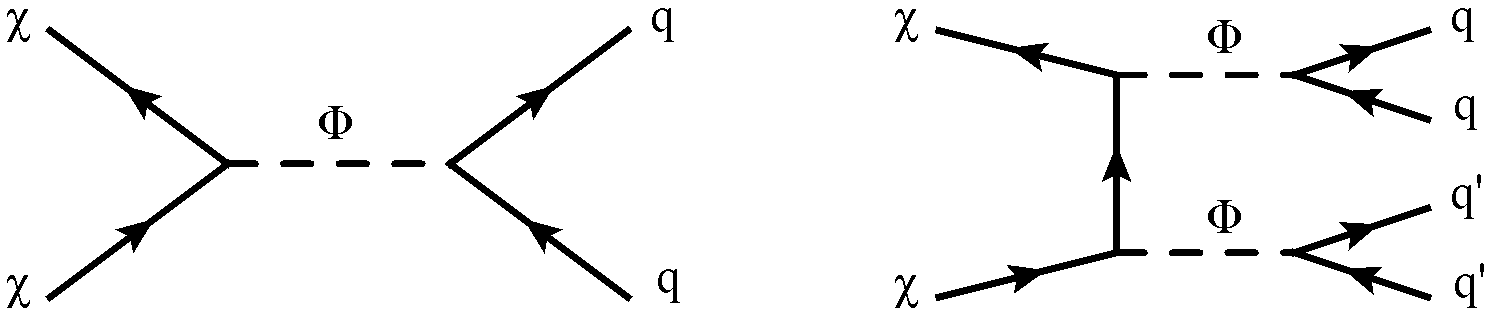
\includegraphics[width=0.78\textwidth]{figures/DMAnnihilationDiagrams.png} 
\vspace{4mm}
\caption{Feynman graphs of 
DM $s$-channel annihilation to quarks (left) and $t$-channel annihilation to a pair of mediators subsequently decaying to quarks (right). The exchanged~$\Phi$ particle(s) can be either (pseudo-)scalar or (axial-)vector mediator(s). 
}
\label{fig:relicprod}
\end{figure}
\end{center}
  
When computing the relic density, we can approximate broad features of the calculation by understanding the form of the leading order production cross section. The leading order cross section can be written as
\begin{align}
  \sigma_{{\rm ann},s}^V \cdot v & = \sum_{q} \frac{N_c^q \hspace{0.125mm} g_{\rm DM}^2 \hspace{0.25mm} g_q^2 \hspace{0.5mm} \beta_q}{2 \pi} \,  \frac{2 m_{\rm DM}^2+ m_q^2}{\left (M_{\rm med}^2 - 4 m_{\rm DM}^2 \right )^2 + M_{\rm med}^2 \Gamma_{\rm med}^2} \,, \label{eq33} \\
\end{align}
for the single mediator vector production, and it can be written as

\begin{align}
  \sigma_{{\rm ann},t}^V \cdot v & =  \frac{ g_{\rm DM}^4   \hspace{0.5mm} \beta_{\rm med}}{4 \pi}  \, \frac{m_{\rm DM}^2 - M_{\rm med}^2 }{\left (M_{\rm med}^2 - 2 m_{\rm DM}^2 \right )^2}  \,, \label{eq37} \\
\end{align}
for the double mediator produdciton.

When we consider single meidator produciton, if we take $ \sigma_{{\rm ann},t}^V \cdot v $ to be propotional to the thermalized cross section obtained from the full relic density calcualtion, and we fix both dark matter mass $m_{\rm DM}$ and mediator mass $M_{\rm med}$, then we have that both equations above can be written in the form of a quadratic equation. Namely, for some constants $A,B,C,D,E,F$, we can write
\begin{align}
A g_{q}^2g_{\rm DM}^2 + B g_{q}^2+Cg_{\rm DM}^2+D g_{q}^4+ E g_{\rm DM}^4+F=0
\end{align}
This also follows from the fact that the widths for standard model particles $\Gamma_{\rm SM}\propto g_{q}^2$, and that the width from dark matter  $\Gamma_{\rm DM}\propto g_{\rm DM}^2$. From this form, we observe that if $g_{\rm DM}$ is a constant, then this equation immediately reduces to a quadratic equation in $g_{q}^2$, and likewise for $g_{\rm DM}^2$ when $g_{q}$ is a constant. Furthermore, the quartic terms $C$ and $D$ are also positive. As a consequence, when all couplings are fixed with the exception of either $g_{q}$ or $g_{\rm DM}$ there is a well defined coupling minimum, and for coupling smaller than the minimum the relic density is larger, and for couplings larger than the minimum. By scanning the couplings, we can find both the minimum and maximum allowed coupling that would satisfy the dark matter relic density.

Figure~\ref{fig:mincoupling} shows the result of a procedure whereby we scan the standard model coupling, compute the relic density and the find the minimum allowed coupling that would not overproduce dark matter. We present this plot for each of the simplified models used within the LHC Dark Matter Working Group. What we find is that for large regons of phase space, in particular light dark matter with a heavy mediator  there is no solution that will produce an underabundance of dark matter. Additionally, we find that couplings of order $g_{q}=1$ are required to statisfy the dark matter relic density for spin 0 scalar and pseudo scalar mediators, and couplings of order $g_{q}=0.1$ or larger are needed to explain spin -1 vector and axial-vector mediators.

The bounds from these models is clearly substantial, and helps to serve as a guide. We would like to stress the fact that as models become more complicated these bounds can change substantially. However, this provides a clear set of benchmarks that can viewed as a target for both invisible, for light dark matter, and visible, for heavy dark matter, searches. 

\begin{figure}[htp!]
  \begin{center}
  \begin{subfigure}[b]{0.49\textwidth}  
    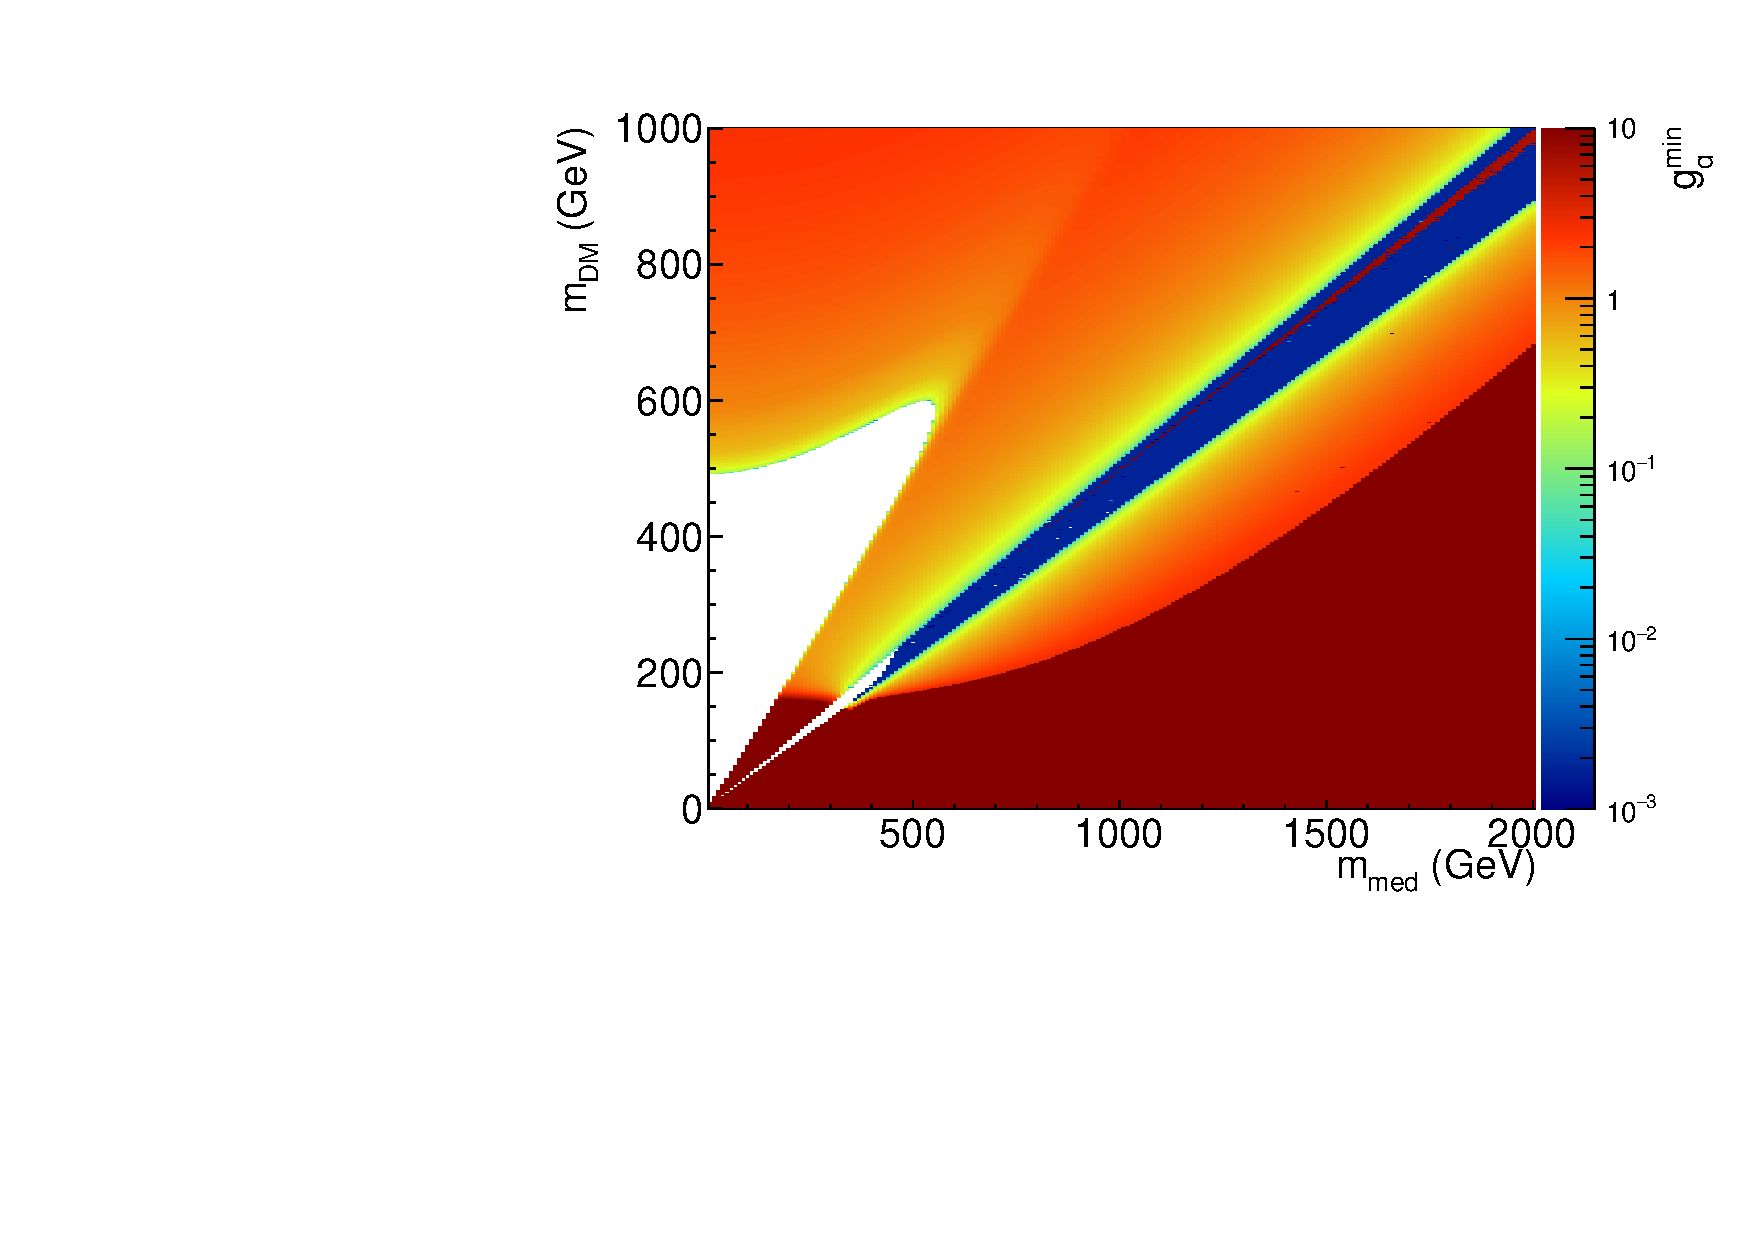
\includegraphics[width=\textwidth]{figures/coupling/s_gqmin.pdf}
    \caption{}
    \label{subfig:scalar}
  \end{subfigure}
  \begin{subfigure}[b]{0.49\textwidth}  
    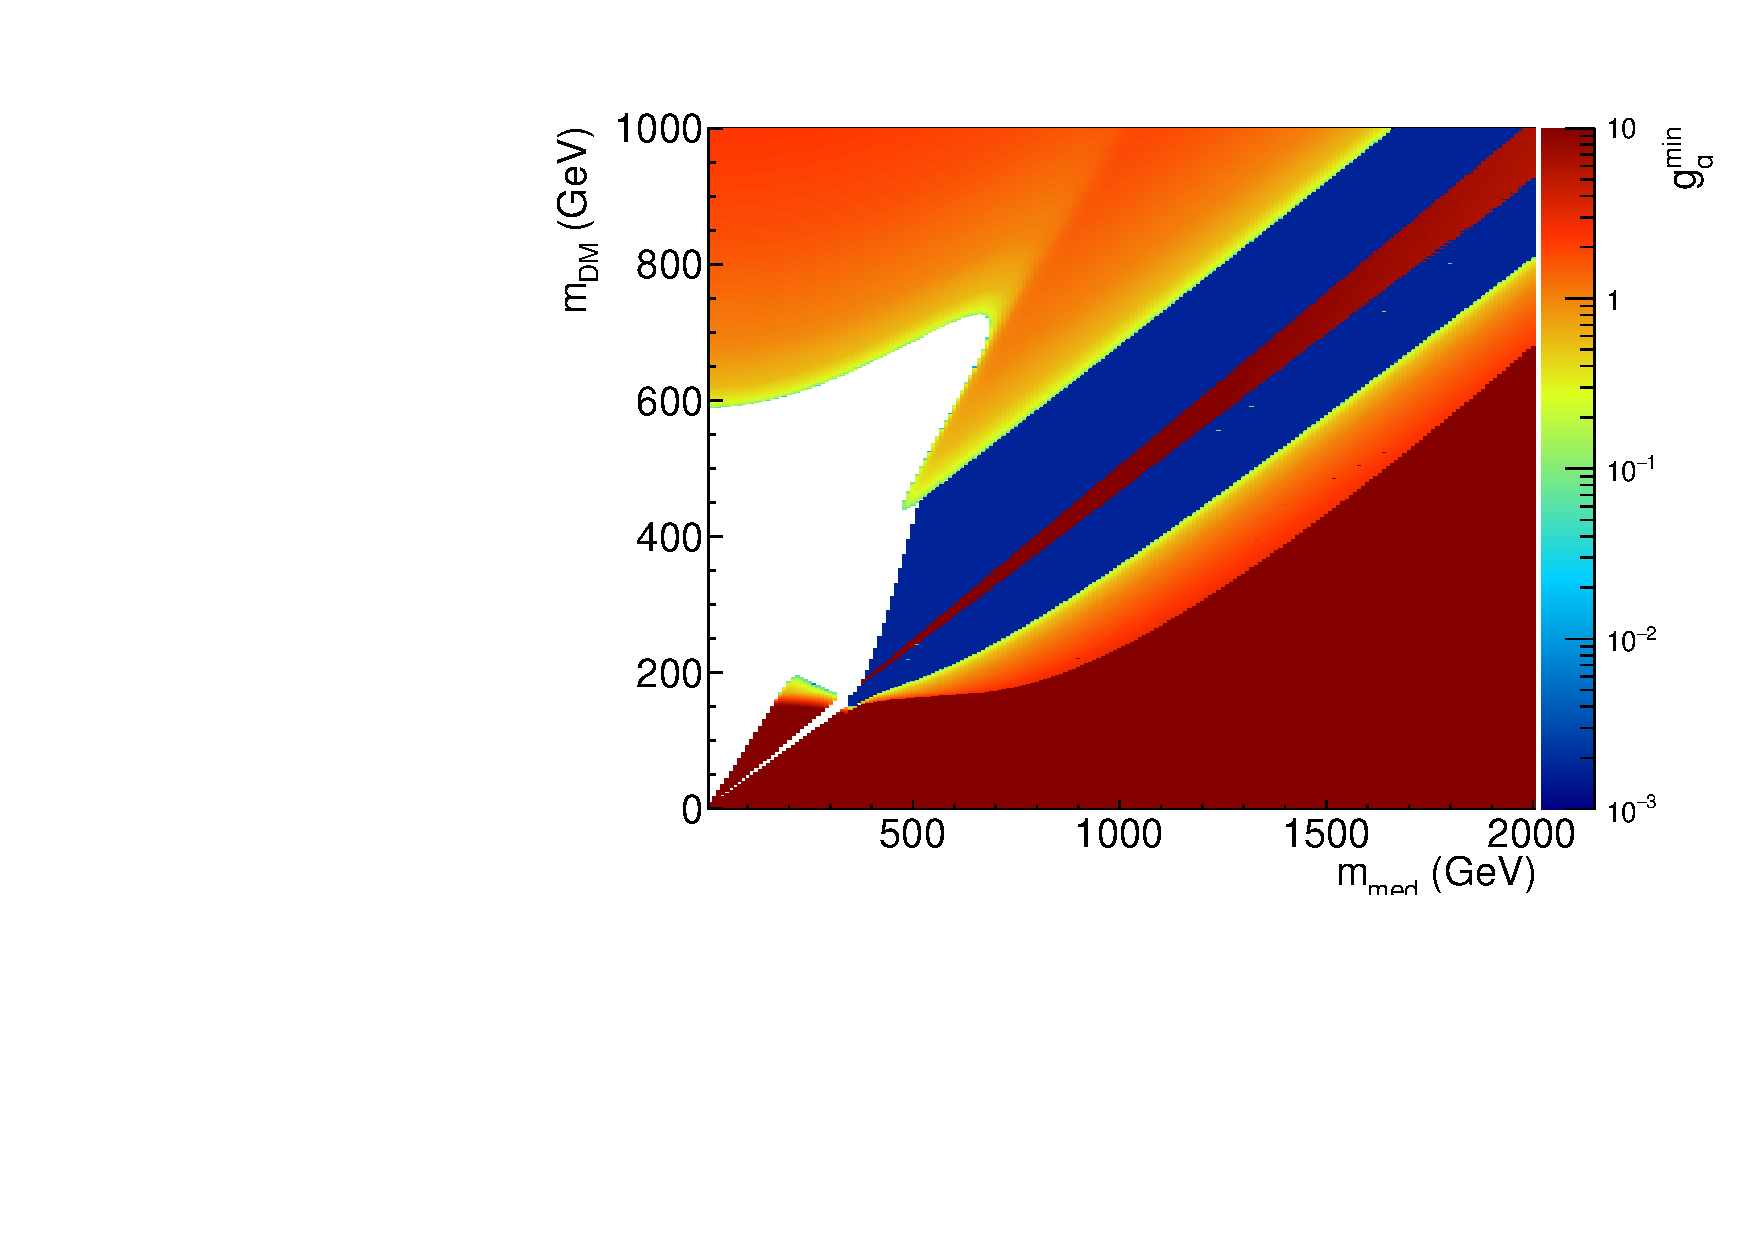
\includegraphics[width=\textwidth]{figures/coupling/p_gqmin.pdf}
    \caption{}
    \label{subfig:pseudoscalar}  
  \end{subfigure}
   \begin{subfigure}[b]{0.49\textwidth}  
    %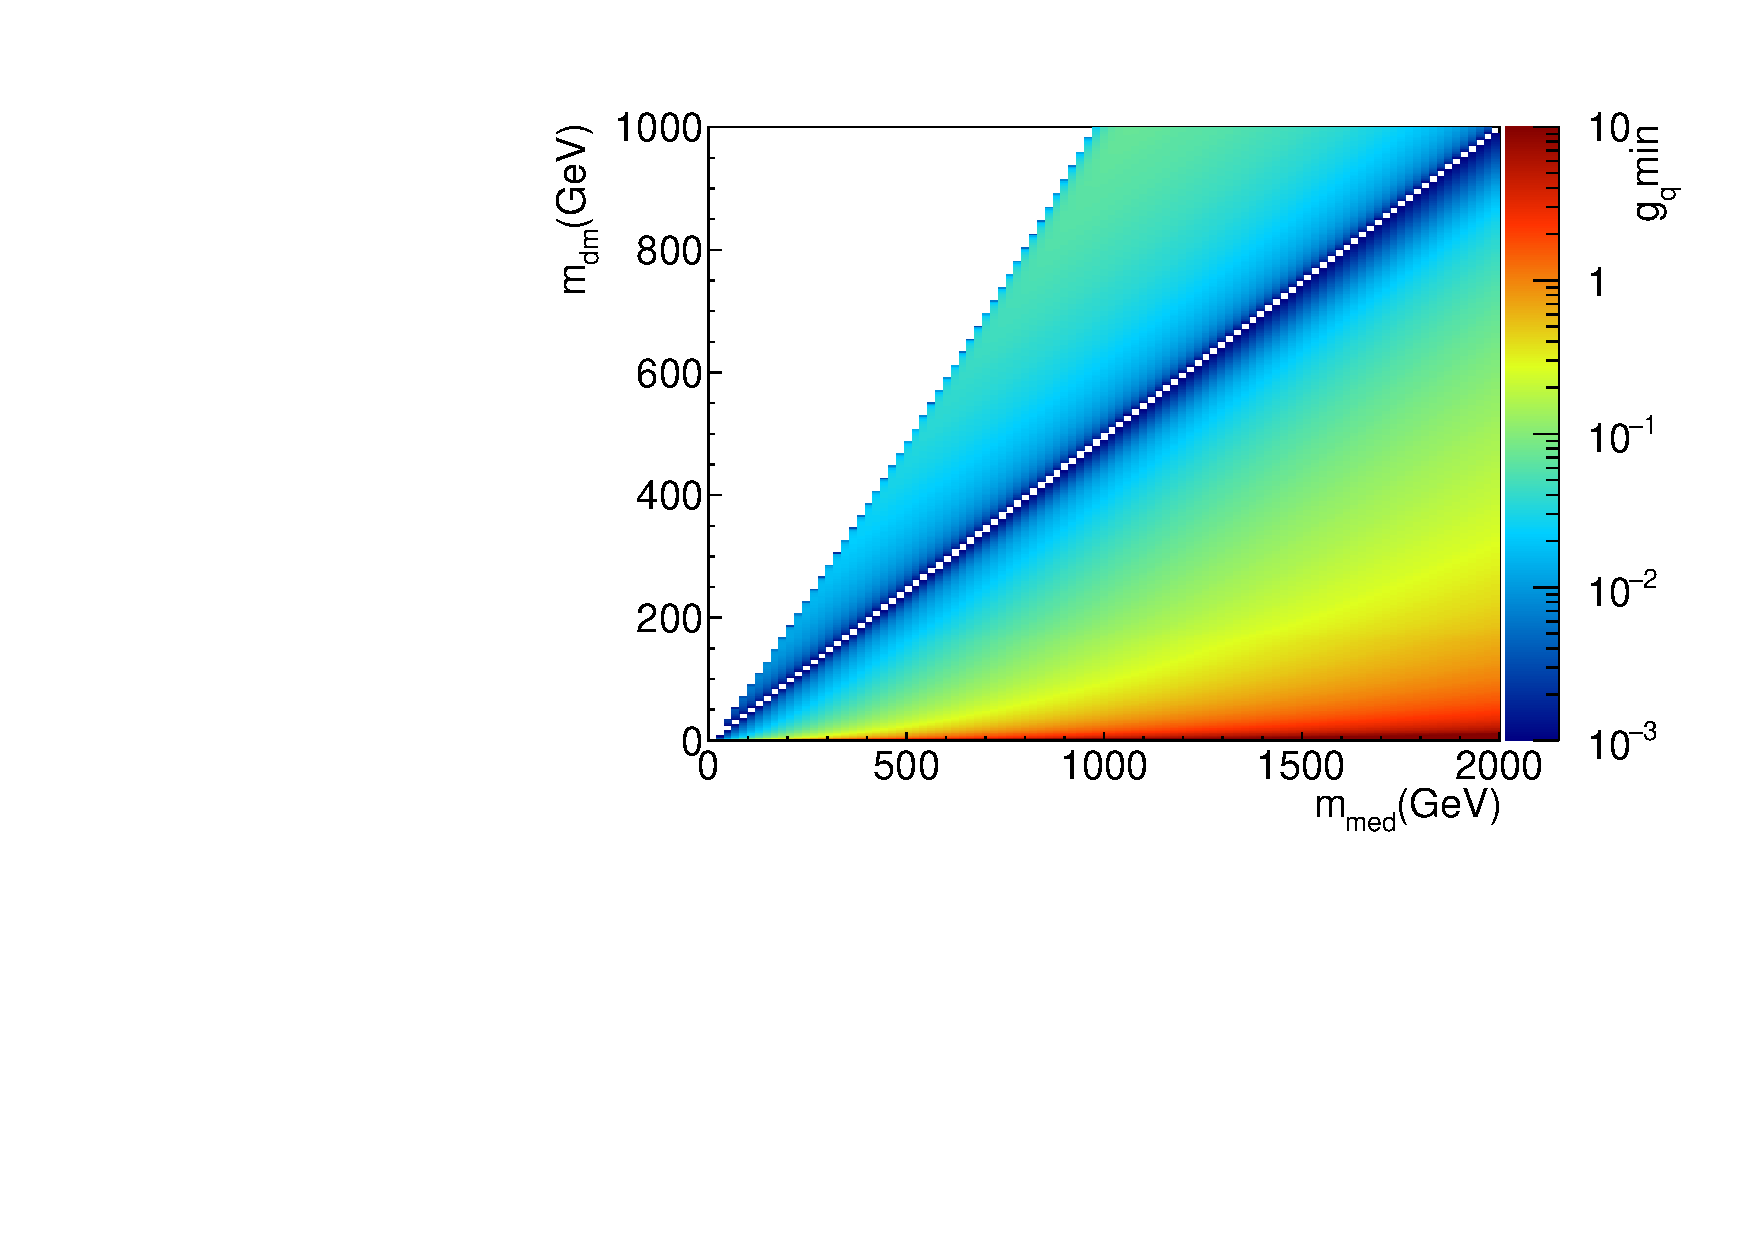
\includegraphics[width=\textwidth]{figures/coupling/v_gqmin.pdf}
    \caption{}
    \label{subfig:vector}
  \end{subfigure}
  \begin{subfigure}[b]{0.49\textwidth}  
    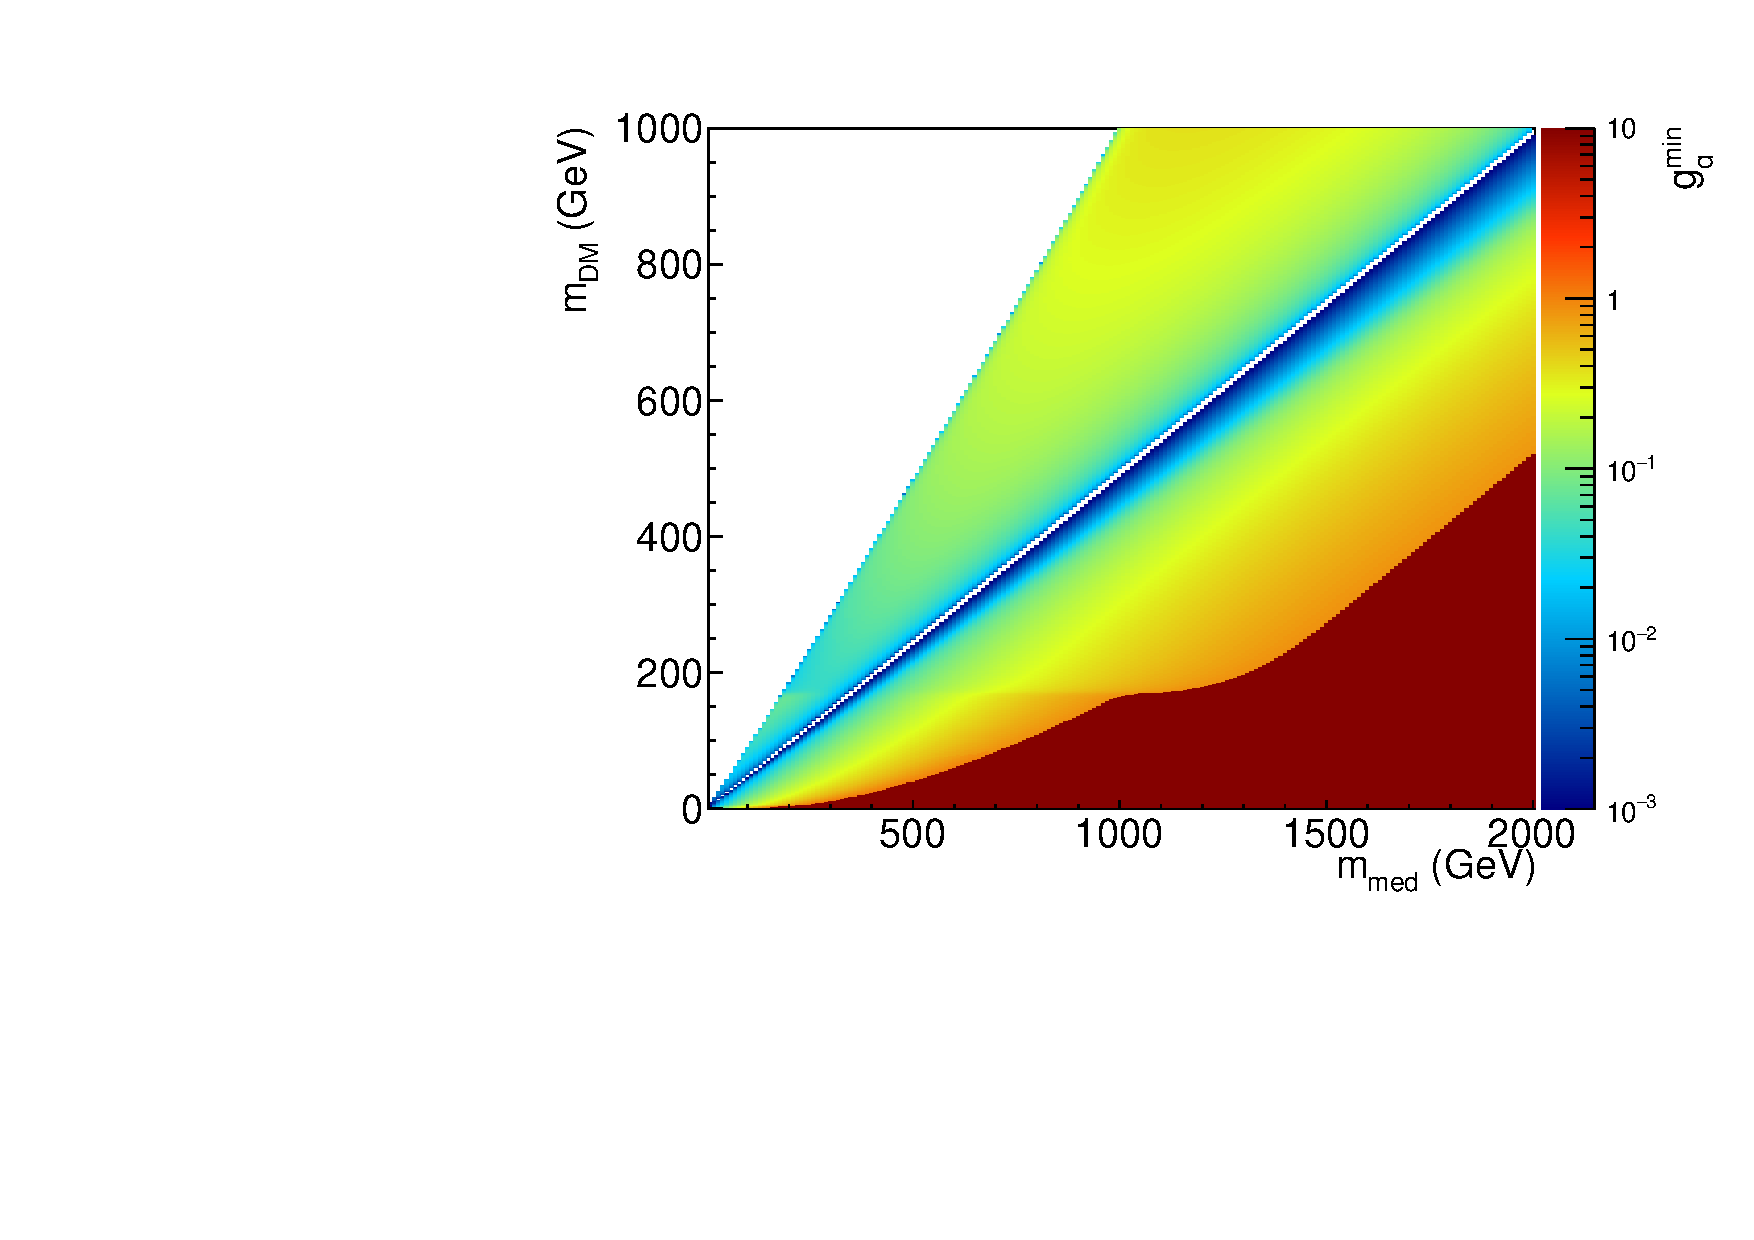
\includegraphics[width=\textwidth]{figures/coupling/a_gqmin.pdf}
    \caption{}
    \label{subfig:axialvector}  
  \end{subfigure}
  \caption{
    Minimum allowed coupling for the scalar (top-left), pseudo-scalar(top-right), axial-vector(bot-left), and vector(bot-right) mediators. The minimum coupling is computed on the z-axis. For the scalar, and pseudoscalar mediators, this coupling is treated as a correction to the yukawa coupling.  
  }
  \label{fig:mincoupling}
  \end{center}
\end{figure}


%%%%%%%%%%%%%%%%%%%%%%%%%%%%%%%%%%%%%%%%%%%%%%%%%%%%%%%%%%%%%%%%%%%%
\section{Conclusion}

% We have demonstrated the way that you can mathematically rescale from AV to V and back, between different couplings, for invisible and visible final states whose LO diagrams are the ones given here.

% Certain caveats to do with acceptances - these are the responsibility of the reader

% Certain caveats to do with k-factors - can make no guarantees so check or sort out an extrapolation if concerned

% Code will be made public with full paper, but you can of course reach out to us for it now, and it is available to members of both ATLAS and CMS already

% Interested in a follow-up that will include scalar and pseudoscalar, but math is quite different.

%%%%%%%%%%%%%%%%%%%%%%%%%%%%%%%%%%%%%%%%%%%%%%%%%%%%%%%%%%%%%%%%%%%%
%%%%%%%%%%%%%%%%%%%%%%%%%%%%%%%%%%%%%%%%%%%%%%%%%%%%%%%%%%%%%%%%%%%%
%%%%%%%%%%%%%%%%%%%%%%%%%%%%%%%%%%%%%%%%%%%%%%%%%%%%%%%%%%%%%%%%%%%%

\acknowledgments 

[To be updated] The research of A.~Boveia is supported by the U.S. DOE grant  DE-SC0011726. C.~Doglioni has received funding from the European Research Council under the European Union's Horizon 2020 research and innovation program (grant agreement 679305) and from the Swedish Research Council. U.~Haisch acknowledges the hospitality and support of the CERN Theoretical Physics Department. The work of T.~M.~P.~Tait is supported in part by NSF grant PHY-1316792. We gratefully acknowledge the support by the U.S. DOE. 

%%%%%%%%%%%%%%%%%%%%%%%%%%%%%%%%%%%%%%%%%%%%%%%%%%%%%%%%%%%%%%%%%%%
%%%%%%%%%%%%%%%%%%%%%%%%%%%%%%%%%%%%%%%%%%%%%%%%%%%%%%%%%%%%%%%%%%%%
%%%%%%%%%%%%%%%%%%%%%%%%%%%%%%%%%%%%%%%%%%%%%%%%%%%%%%%%%%%%%%%%%%%%

% KP: for the "real" paper we should include an appendix documenting the code usage but for this stage we are not ready to document the code, so we don't need an appendix
% \appendix

% \section{Appendix}
% \label{app:recast}

% Document public code here?

\newpage 

\bibliography{CouplingScan-whitepaper}
\bibliographystyle{JHEP}



\end{document}
